\newcommand{\duedate}{17 September 2026}
\documentclass{16384_doc}
\usepackage{enumitem}
\usepackage{tikz}
\usetikzlibrary{positioning,arrows,arrows.meta,matrix,fit,backgrounds,calc,math,patterns,patterns.meta,intersections,fpu}
\newcommand{\assignmentname}{Assignment 2: Jacobians}

\begin{document}
\maketitle

\tableofcontents

\section{Theory Questions}

\begin{questions}
    \titledquestion{PR Arm}[20]
    Use the PR Arm illustrated below from Assignment 1. The rotary joint $\varphi$ measures the bearing angle, so $\varphi=0$ means the arm is pointing straight up. The illustration shows the arm around $\varphi=\pi/4$ with $d=1$ and $l_1=1$.

    \begin{center}
        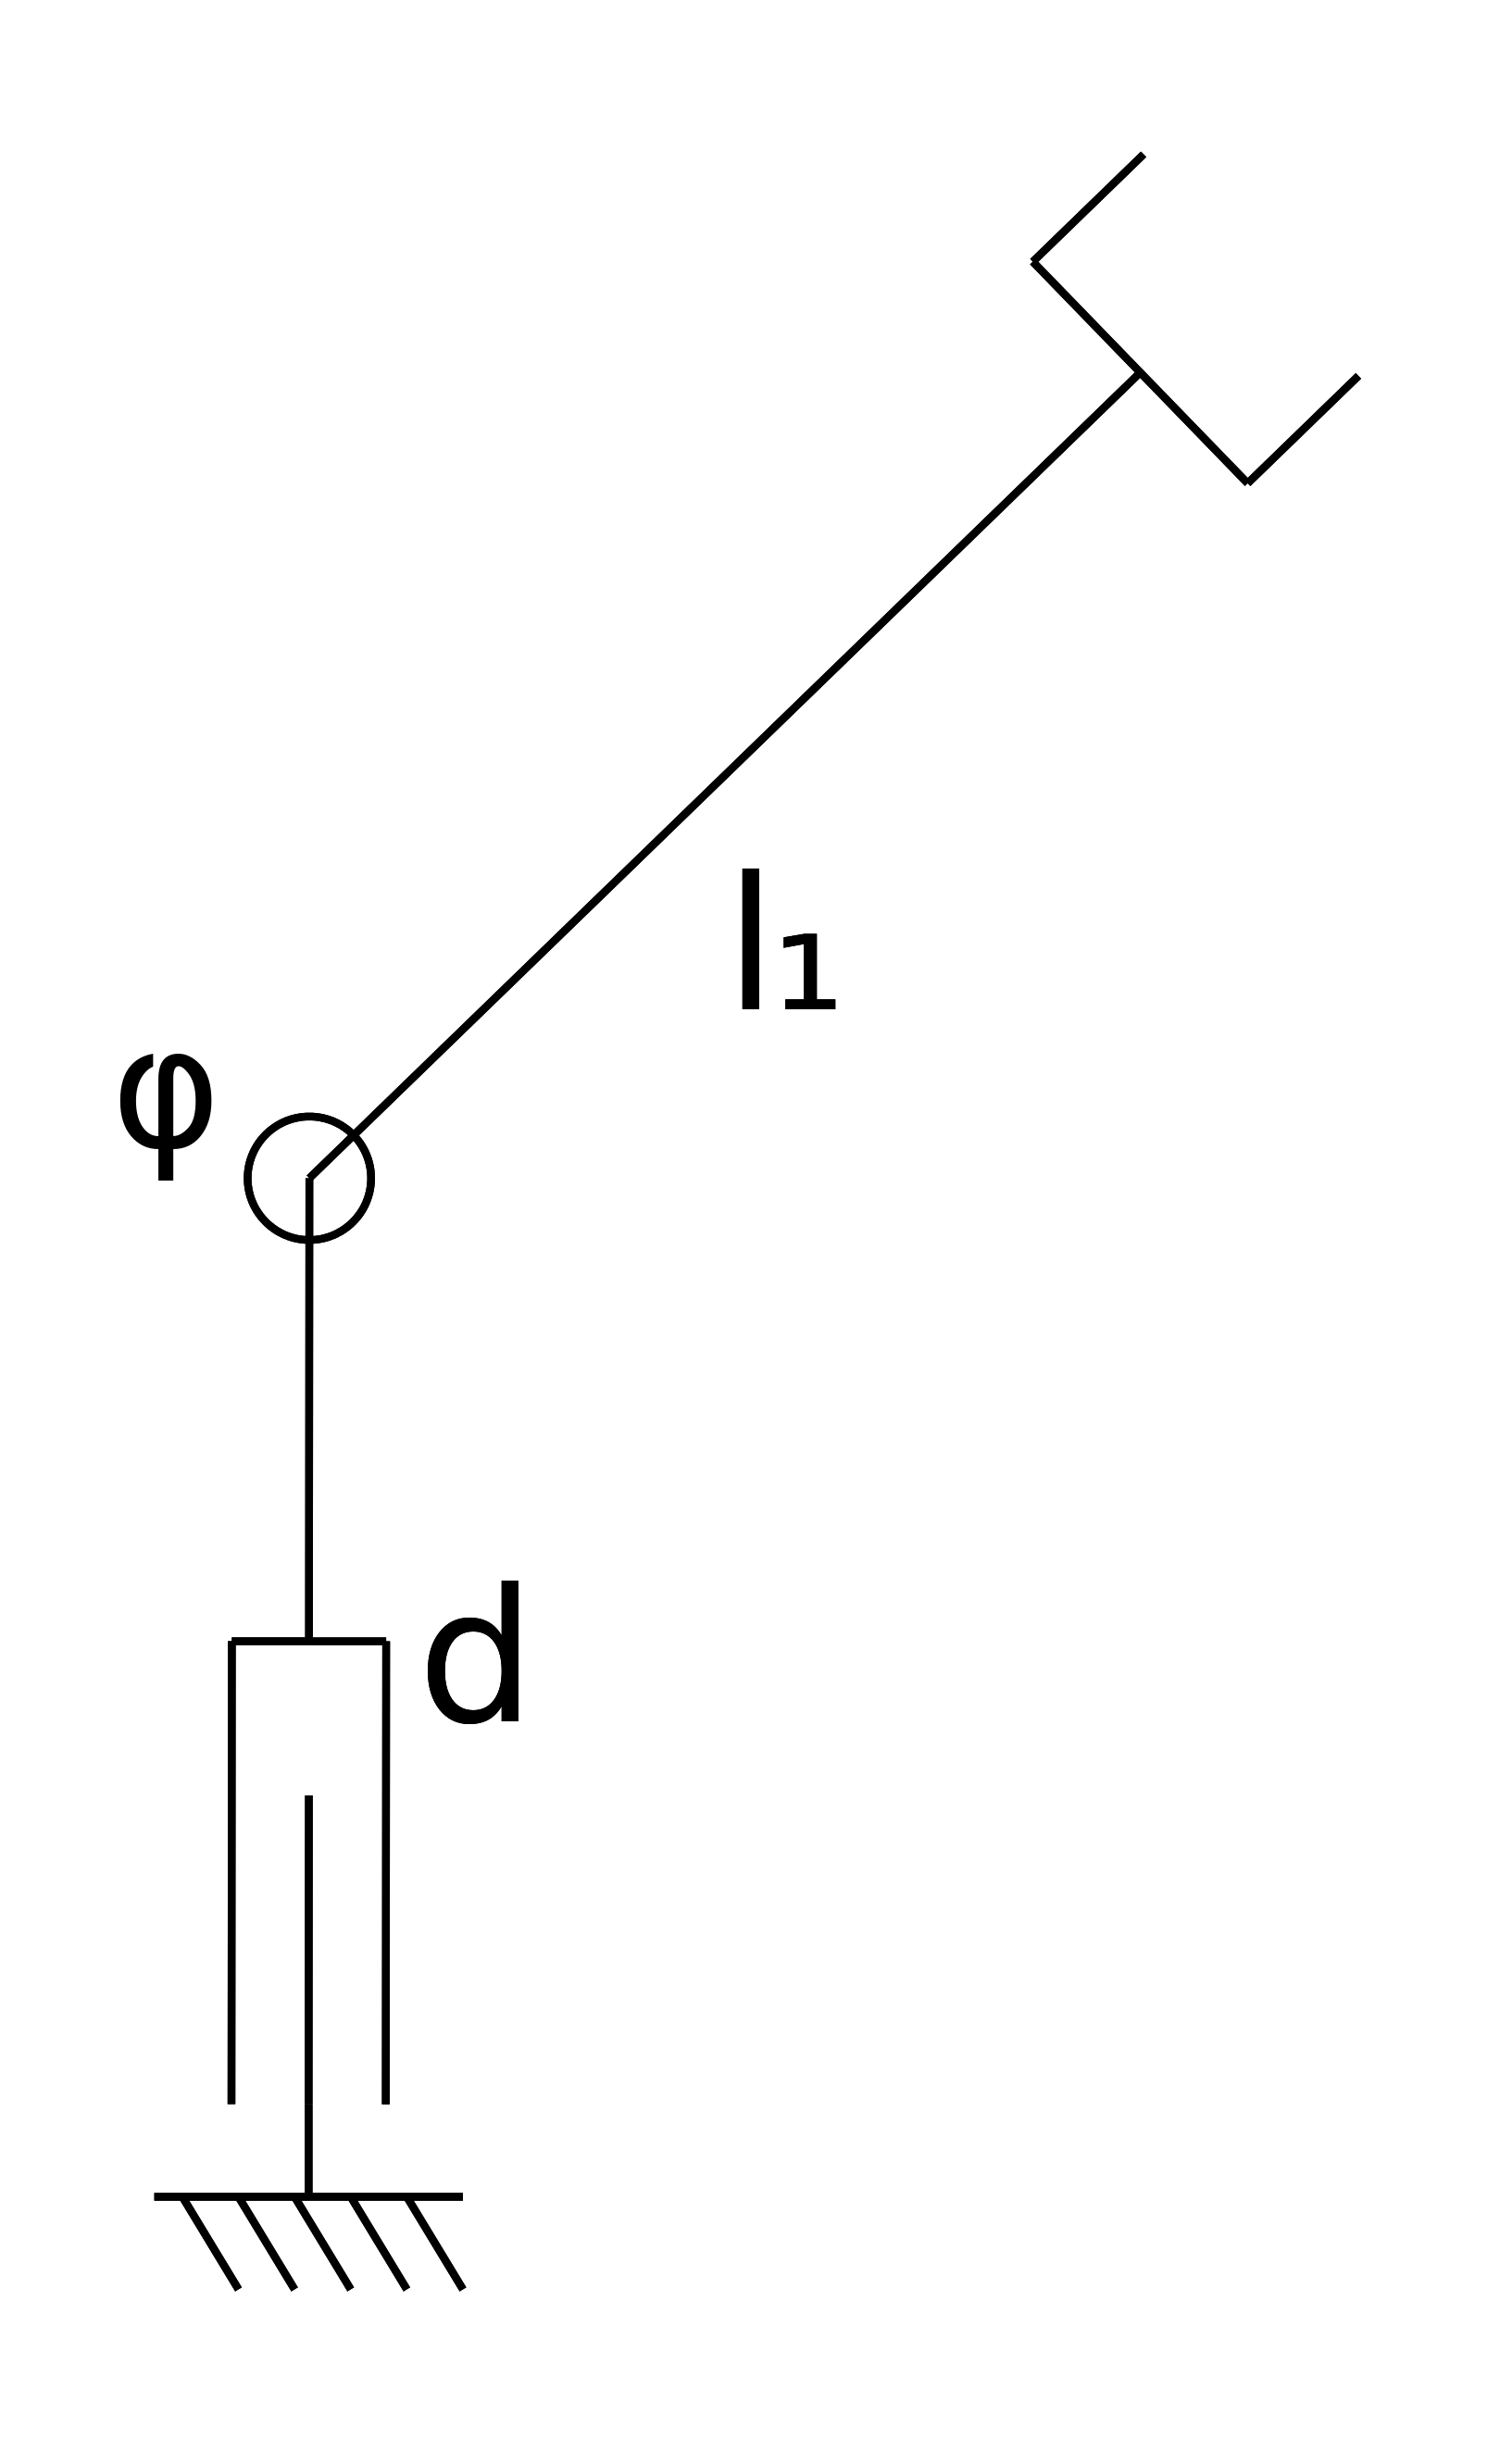
\includegraphics[width=1.5in]{generated_figures/robot_7_2.png}
    \end{center}

    \begin{enumerate} [label=\alph*.]
        \item \text{[1 point]} What is the dimension of the end-effector Jacobian $J$?\  Assume the workspace is $SE(2)$.
        \begin{tcolorbox}[height=3cm]
        % TODO: ENTER YOUR ANSWER HERE
        \end{tcolorbox}

        \item \text{[1 points]} What does each row of $J$ mean (in 1--2 sentences)?
        \begin{tcolorbox}[height=3cm]
        % TODO: ENTER YOUR ANSWER HERE
        \end{tcolorbox}

        \item \text{[1 points]} What does each column of $J$ mean (in 1--2 sentences)?
        \begin{tcolorbox}[height=3cm]
        % TODO: ENTER YOUR ANSWER HERE
        \end{tcolorbox}
        \vspace{1em}

        \item \text{[2 points]} Find the forward-kinematic map to the end effector for this arm for $x$, $y$, and $\th$ as a function $f(d, \varphi)$. Check that the coordinates match the figure above for $d=1$ and $\varphi=\pi/4$.
        \begin{tcolorbox}[height=3cm]
        % TODO: ENTER YOUR ANSWER HERE
        \end{tcolorbox}

        \item \text{[5 points]} Determine the Jacobian of the arm by taking the partial derivatives of the forward-kinematic map with respect to $d$ and $\varphi$.
        \begin{tcolorbox}[height=3cm]
        % TODO: ENTER YOUR ANSWER HERE
        \end{tcolorbox}

        \item \text{[5 points]} Let $d = 0$, $\varphi = 0$ and $\dot{d} = \dot{\varphi} = v$, what is the contribution of each joint to the end-effector's linear velocity? To the angular velocity?
        \begin{tcolorbox}[height=3cm]
        % TODO: ENTER YOUR ANSWER HERE
        \end{tcolorbox}

        \item \text{[5 points]} For this problem, assume that forces due to gravity are
        pointing in the negative $y$ direction. Assume each \textbf{link} has a mass of
        0.5\,kg and the center of mass is in the center of that link.
        \begin{enumerate} [label=(\roman*)]
        \item What are the efforts
        (as a function of the configuration $\Theta=\smcolvec{d\\\varphi}$) necessary to counteract the effect
        of gravity on the first link? Assume all of the first link's mass is on the distal end of the prismatic joint.
        \item Of link $l_1$?
        \item What efforts are necessary to counteract the effect of gravity on all both links at the same time?
        \end{enumerate}
        \begin{tcolorbox}[height=3cm]
        % TODO: ENTER YOUR ANSWER HERE
        \end{tcolorbox}

    \end{enumerate}

    \pagebreak
    \titledquestion{Robot Analysis: RRR}[30]
    Consider the following robot. Assume no joint limits, and that the links lengths are $l_1=l_2=l_3=1$. The joint angles are measured as a relative angle from the previous link / horizontal, so $\th[1]=\th[2]=\th[3]=0$ means the arm is fully extended to the right. Note that positive angles rotate counter-clockwise, unlike problem 1.

    \begin{center}
    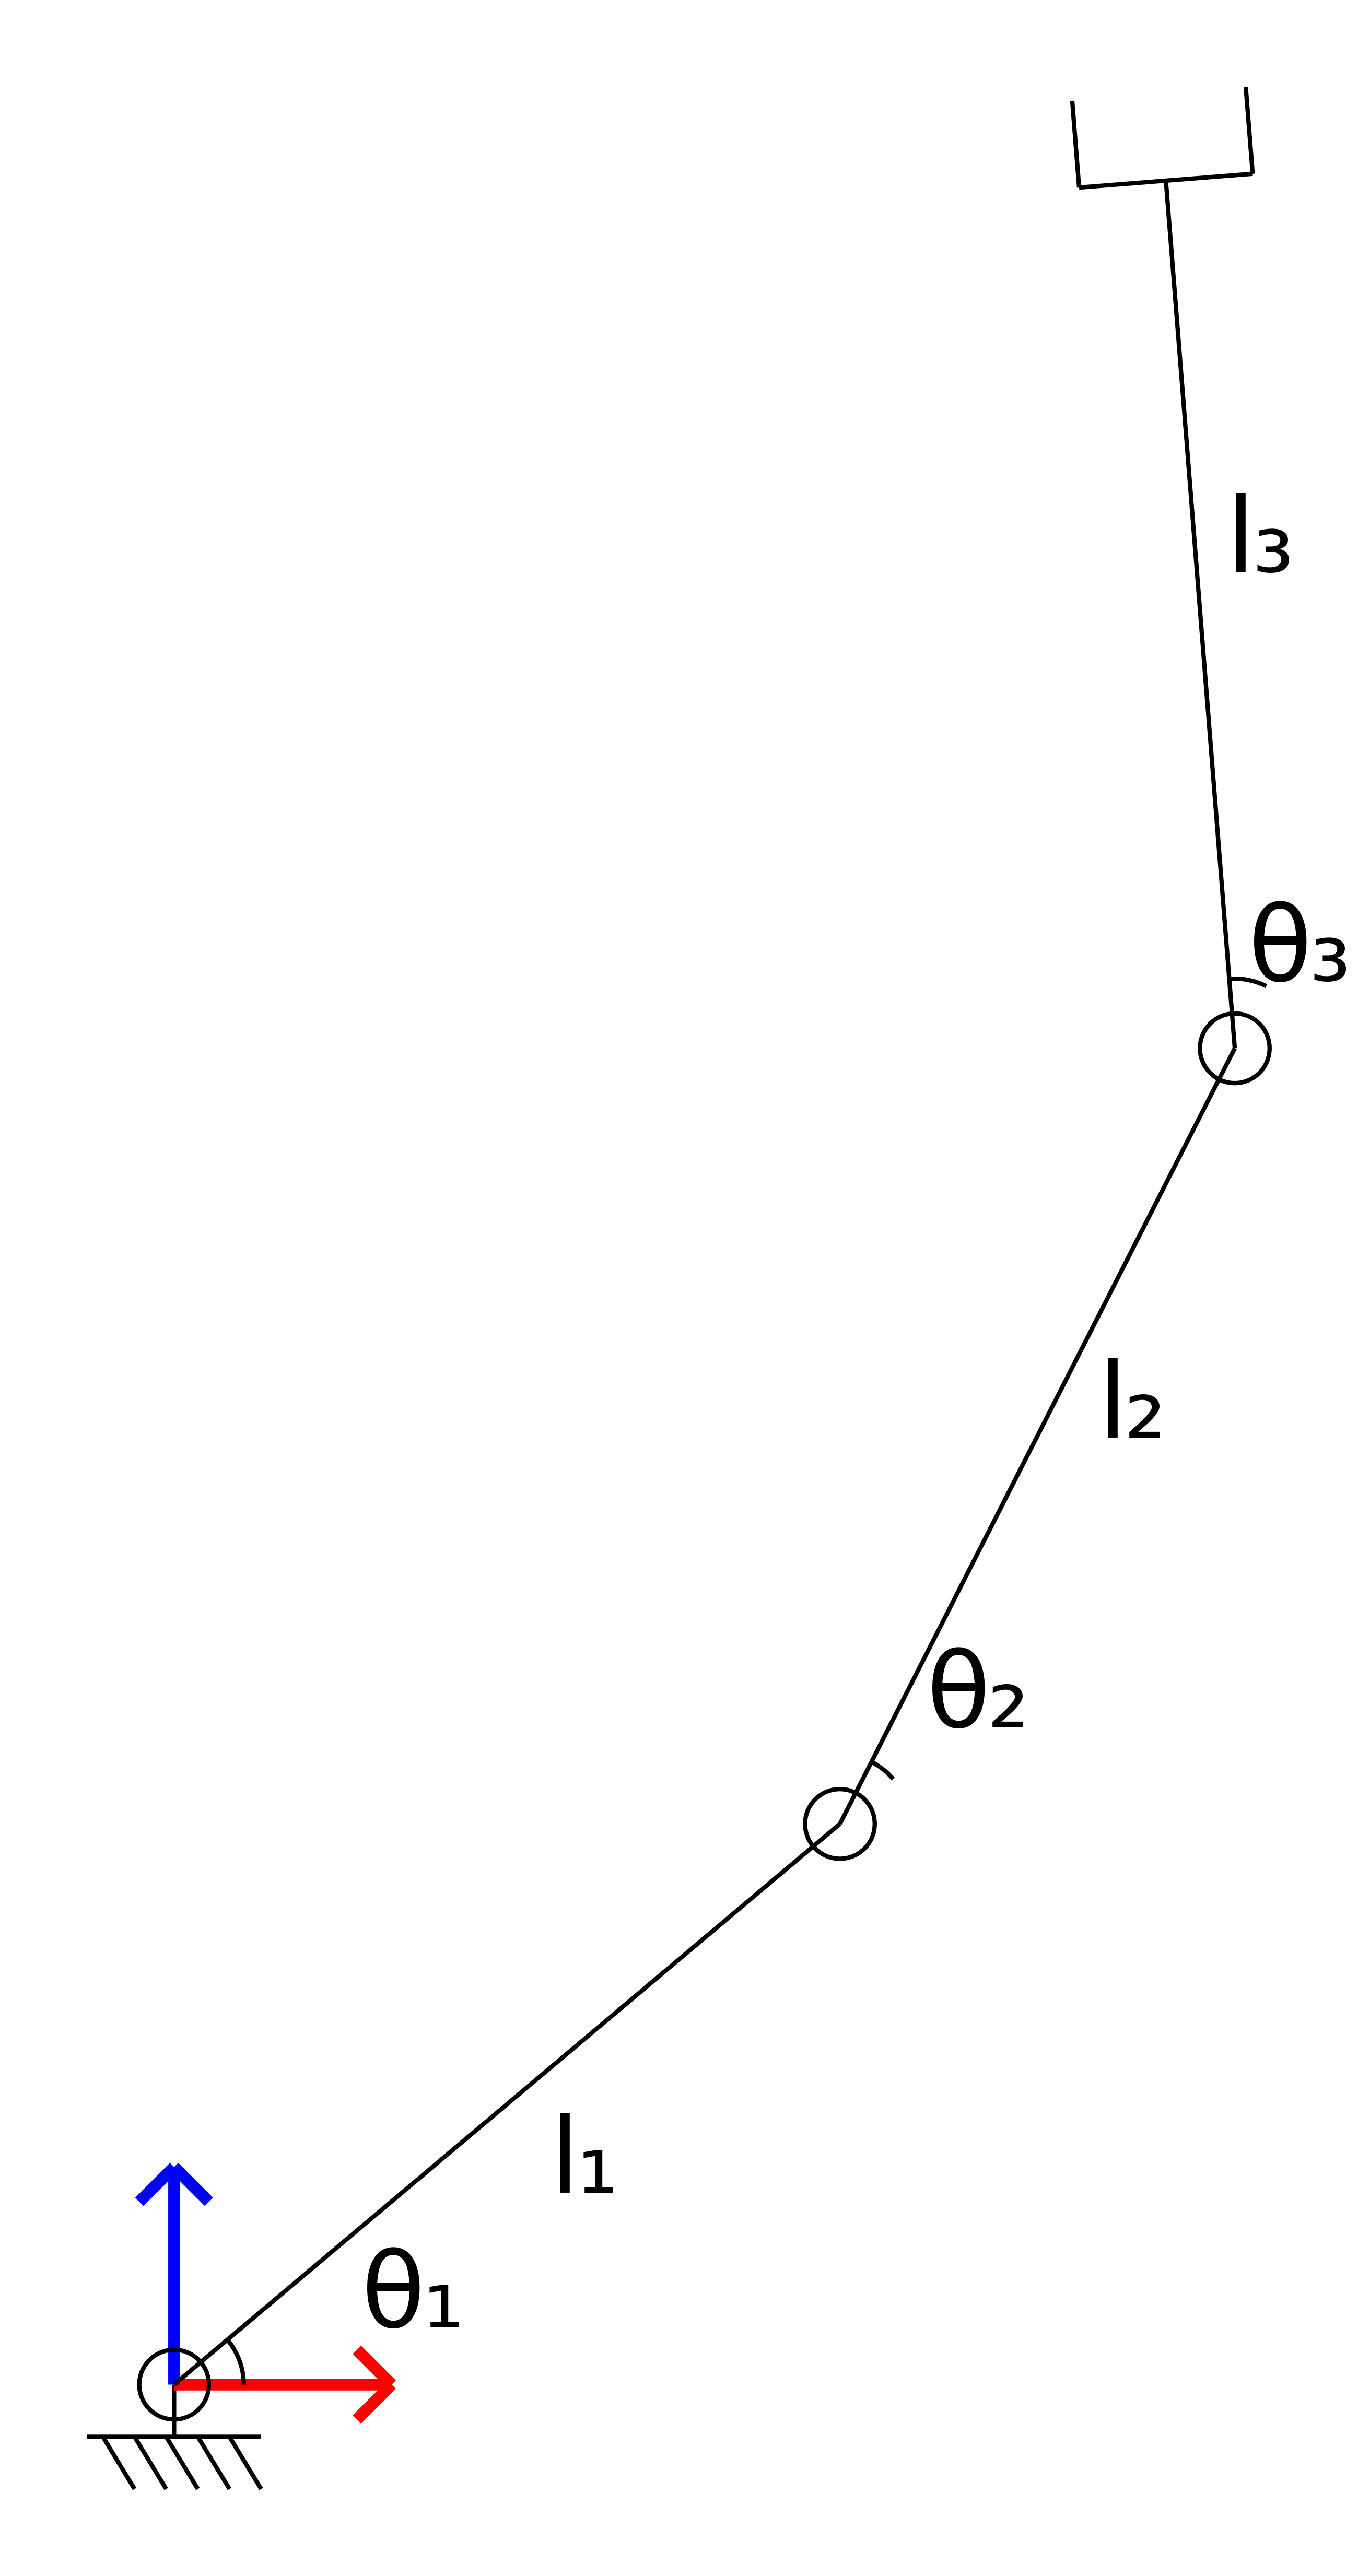
\includegraphics[scale=0.07]{generated_figures/robot_1.png}
    \end{center}

    \begin{enumerate} [label=\alph*.]
        \item \text{[8 points]} Find the Jacobian for the end effector as a function of the joint angles $\th[1]$, $\th[2]$, and $\th[3]$.  Assume the workspace is $SE(2)$.
        \begin{tcolorbox}[height=3cm]
        % TODO: ENTER YOUR ANSWER HERE
        \end{tcolorbox}

        \item \text{[2 point]} Is this robot ever singular? If so, when?
        \begin{tcolorbox}[height=2cm]
        \end{tcolorbox}

        \item \text{[5 points]} When the arm is at
        position $(\th[1], \th[2], \th[3]) = (0, 0, \pi/2)$, and $\thd[1] = \thd[2] = \thd[3] =
        v$, what is the contribution of each joint to the end-effector's
        linear velocity?  To the angular velocity?
        \begin{tcolorbox}[height=3cm]
        % TODO: ENTER YOUR ANSWER HERE
        \end{tcolorbox}

        \item \text{[5 points]} At configuration $\th[1] = \th[2] = \th[3] = 0$,
        \begin{enumerate} [label=(\roman*)] 
            \item Is this configuration singular? Why or why not?
            \item What \smcolvec{\thd[1]\\\thd[2]\\\thd[3]} can be applied to instantaneously move the end-effector in the planar direction \smcolvec{0\\1}?
            \item How about \smcolvec{1\\0}?
            \item With rotation, what joint velocities must be applied to move instantaneously in \smcolvec{0\\ 1\\ 1}, where the third term is rotation?
        \end{enumerate}
        \begin{tcolorbox}[height=6cm]
        % TODO: ENTER YOUR ANSWER HERE
        \end{tcolorbox}

        \item \text{[5 points]} At configuration $(\th[1], \th[2], \th[3]) = (0, \pi/2, 0)$, what joint torques are necessary to exert a wrench of \smcolvec{1\\0\\1}?
        \begin{tcolorbox}[height=3cm]
        % TODO: ENTER YOUR ANSWER HERE
        \end{tcolorbox}

        \item \text{[5 points]} For this problem, assume that forces due to gravity are
        pointing in the negative $y$ direction.  Assume each \textbf{link} has a mass of
        1\,kg and the center of mass is in the center of that link. 
        \begin{enumerate} [label=(\roman*)]
            \item What are the joint torques (as a function of the configuration $\Theta=\smcolvec{\th[1]\\\th[2]\\\th[3]}$) necessary to counteract the effect of gravity on the center of mass of link $l_1$?
            \item Of link $l_2$?
            \item Of link $l_3$?
            \item What torques are necessary to counteract the effect of gravity on all three links
            at the same time?
        \end{enumerate}
        \begin{tcolorbox}[height=3cm]
        % TODO: ENTER YOUR ANSWER HERE
        \end{tcolorbox}
    \end{enumerate}

    \pagebreak
    \titledquestion{Robot Analysis: RPRP Arm}[25]
    Consider the following robot (assume no joint limits, and that the links
    do not intersect with the ground):

    \begin{center}
    
\includegraphics[width=0.45\textwidth]{generated_figures/robot_8.png}
    \end{center}

    \begin{enumerate} [label=\alph*.]
        \item \text{[5 points]} Find the forward kinematic map for the end effector.
        \begin{tcolorbox}[height=3cm]
        % TODO: ENTER YOUR ANSWER HERE
        \end{tcolorbox}

        \item \text{[5 points]} Find the Jacobian for the end effector.
        \begin{tcolorbox}[height=5cm]
        % TODO: ENTER YOUR ANSWER HERE
        \end{tcolorbox}

        \item \text{[5 points]} For this problem, assume that forces due to gravity are pointing in the negative $y$ direction. Each link's mass is negligible (0\,kg) and the end effector has a mass of 100\,kg. Calculate the joint torques/efforts (as a function of the configuration $\Theta=\smcolvec{\theta_1\\\theta_2\\d_1\\d_2}$) necessary to counteract the effect of gravity.
        \begin{tcolorbox}[height=3cm]
        % TODO: ENTER YOUR ANSWER HERE
        \end{tcolorbox}

        \item \text{[5 points]} At the configuration $(\th[1], \th[2], d_1, d_2) = (0, \pi/2, 1, 1)$, suppose we have joint torques/efforts of $(\tau_{\th[1]}, \tau_{\th[2]}, \tau_{d_1}, \tau_{d_2})=(-1,-1,1,0)$ applied to the robot's joints. Solving the formula $\tau = J^\top f$ (if possible), what is the wrench at the end effector?  What does this mean physically?
        \begin{tcolorbox}[height=3cm]
        % TODO: ENTER YOUR ANSWER HERE
        \end{tcolorbox}

        \item \text{[5 points]} At the configuration $(\th[1], \th[2], d_1, d_2) = (0, \pi/2, 1, 1)$, suppose we have joint torques/efforts of $(\tau_{\th[1]}, \tau_{\th[2]}, \tau_{d_1}, \tau_{d_2})=(1,0,0,0)$ applied to the robot's joints. Solving the formula $\tau = J^\top F$ (if possible), what is the wrench at the end effector?  What does this mean physically?
        \begin{tcolorbox}[height=3cm]
        % TODO: ENTER YOUR ANSWER HERE
        \end{tcolorbox}
    \end{enumerate}
\end{questions}

\section{Code Questions}

In these problems, we'll analytically test some of the work from the previous section. There is a provided \verb|autograder.py| script which will check your code locally for correctness.

\begin{questions}
    \setcounter{question}{3}
    \titledquestion{Jacobians and Velocities}[25]
        Begin by opening the \verb!ex1! directory in your Python environment. In this exercise, you must fill out several Python files. When completed correctly, the first three functions will define the forward kinematics and Jacobian to several points on an RR arm; the final function will provide a self-check for the first three functions.
        \begin{center}
        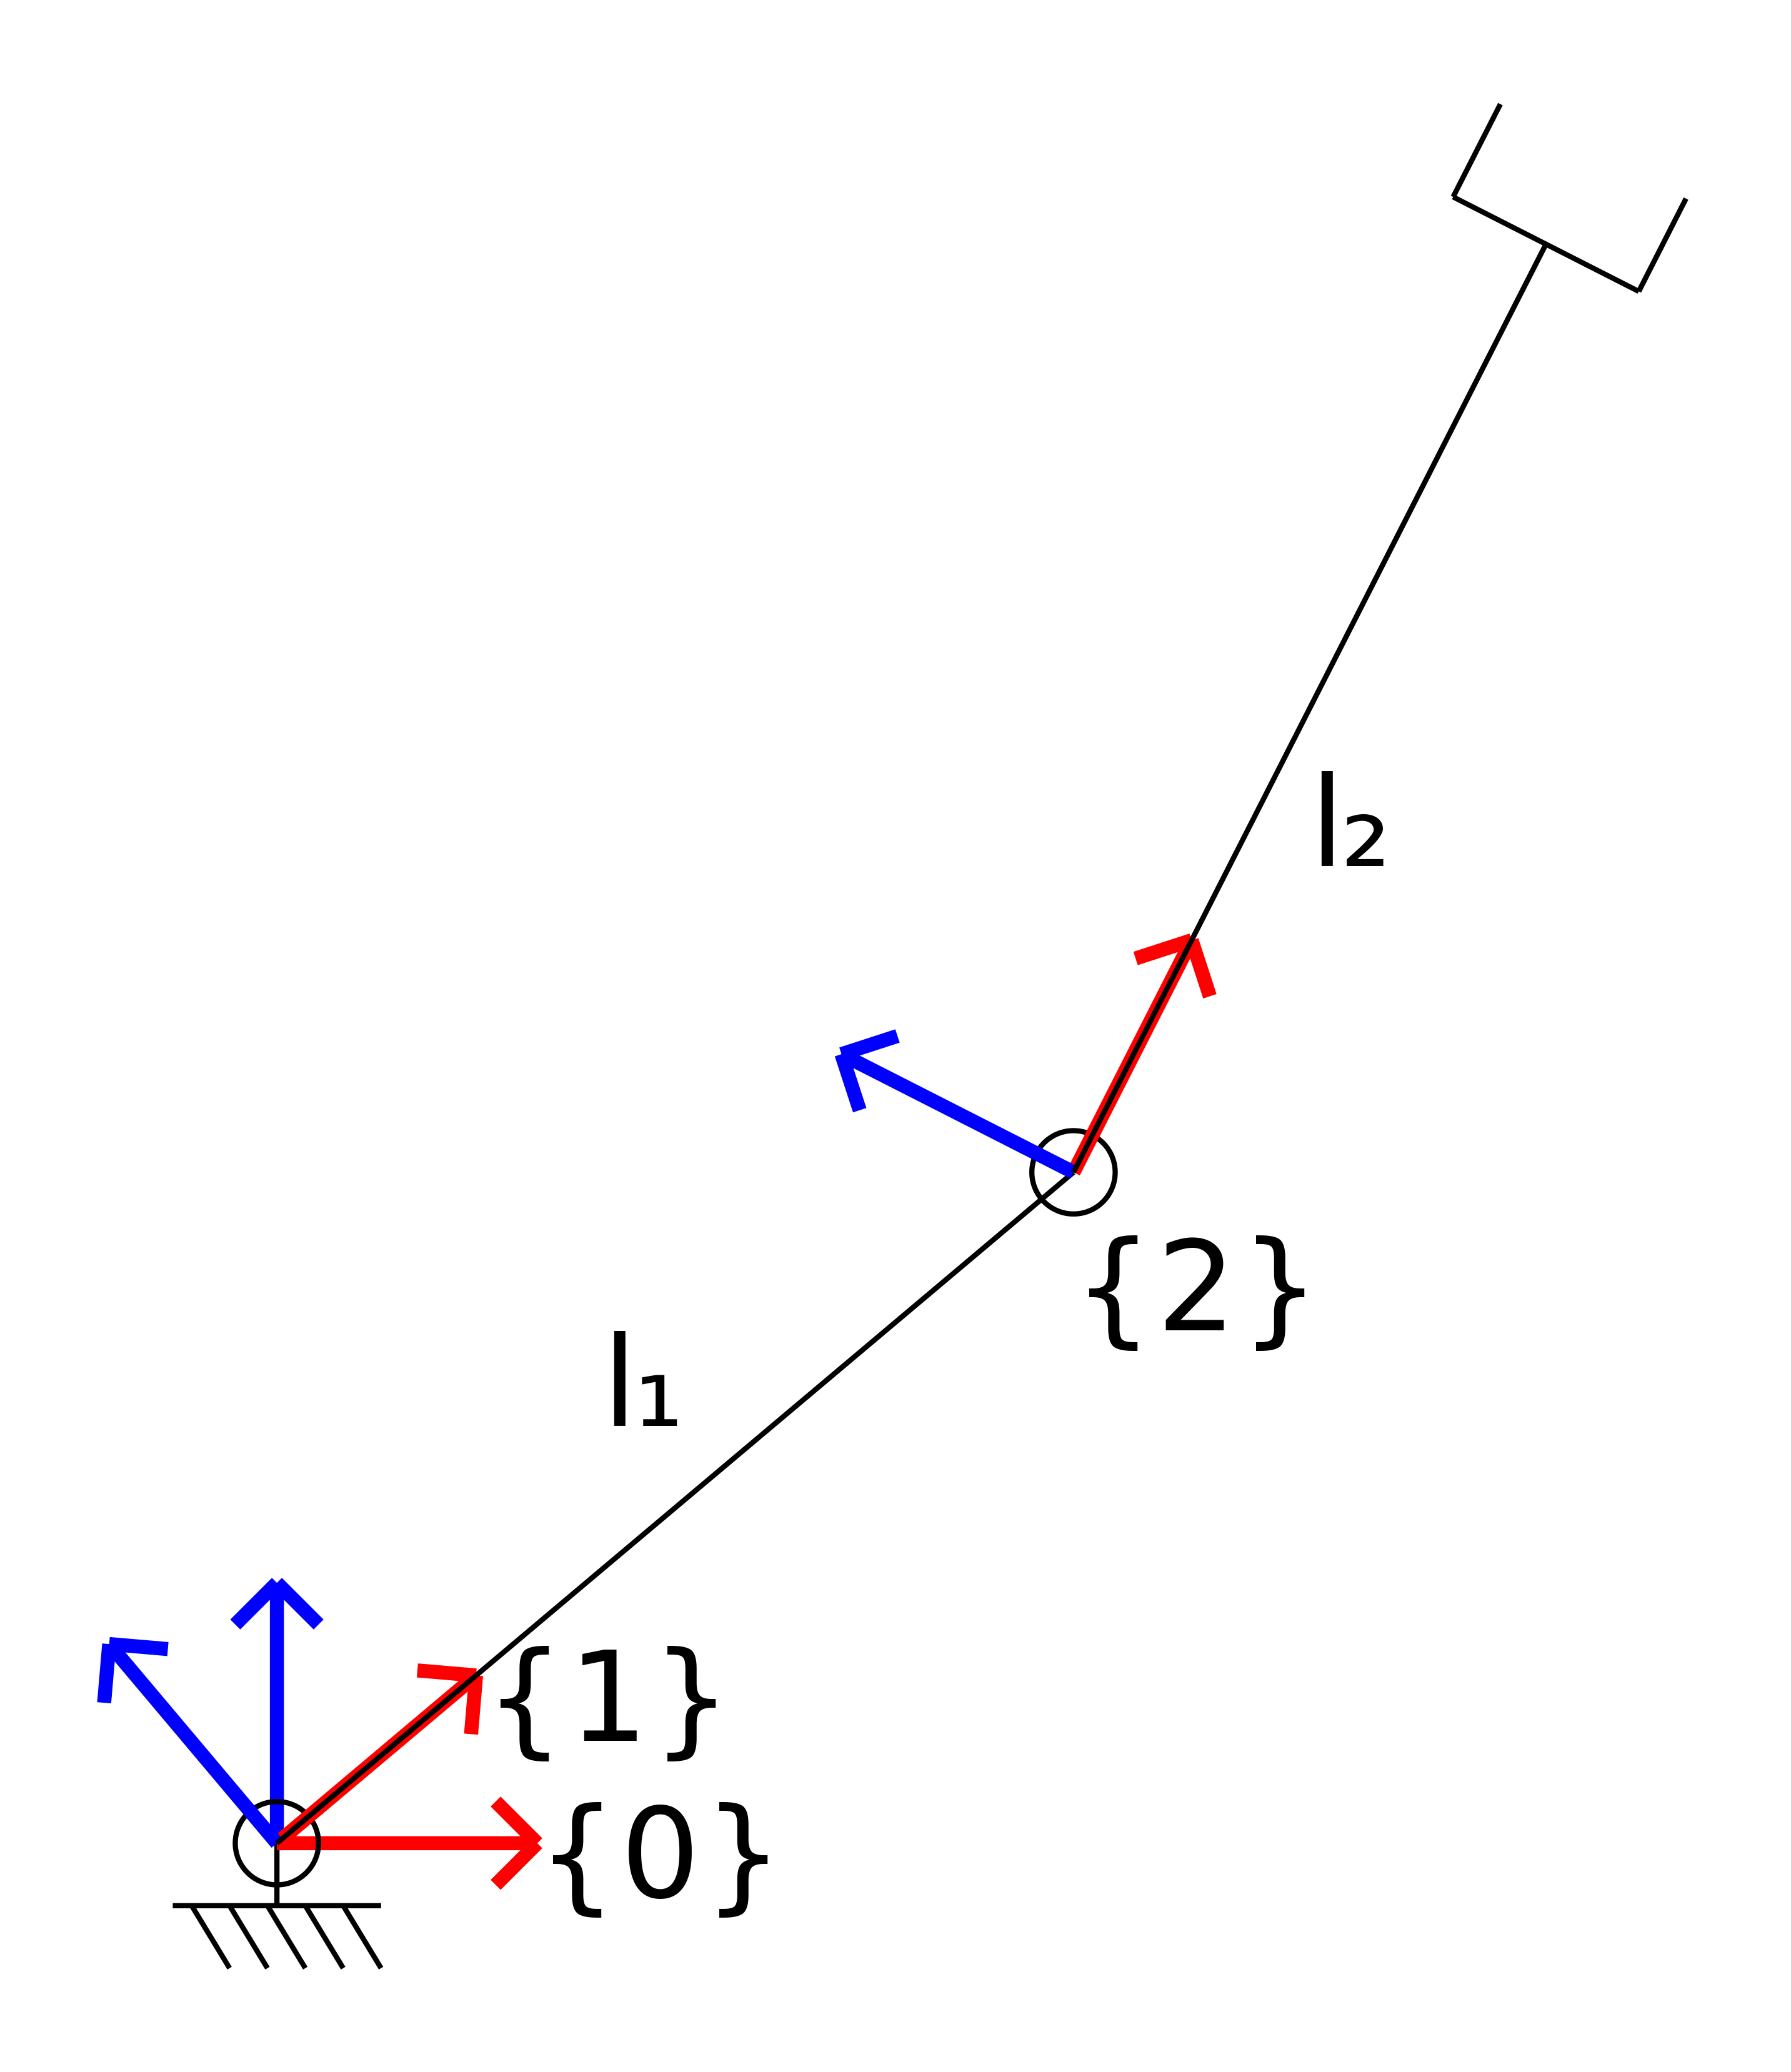
\includegraphics[scale=0.05]{generated_figures/code_1_FK.png}
        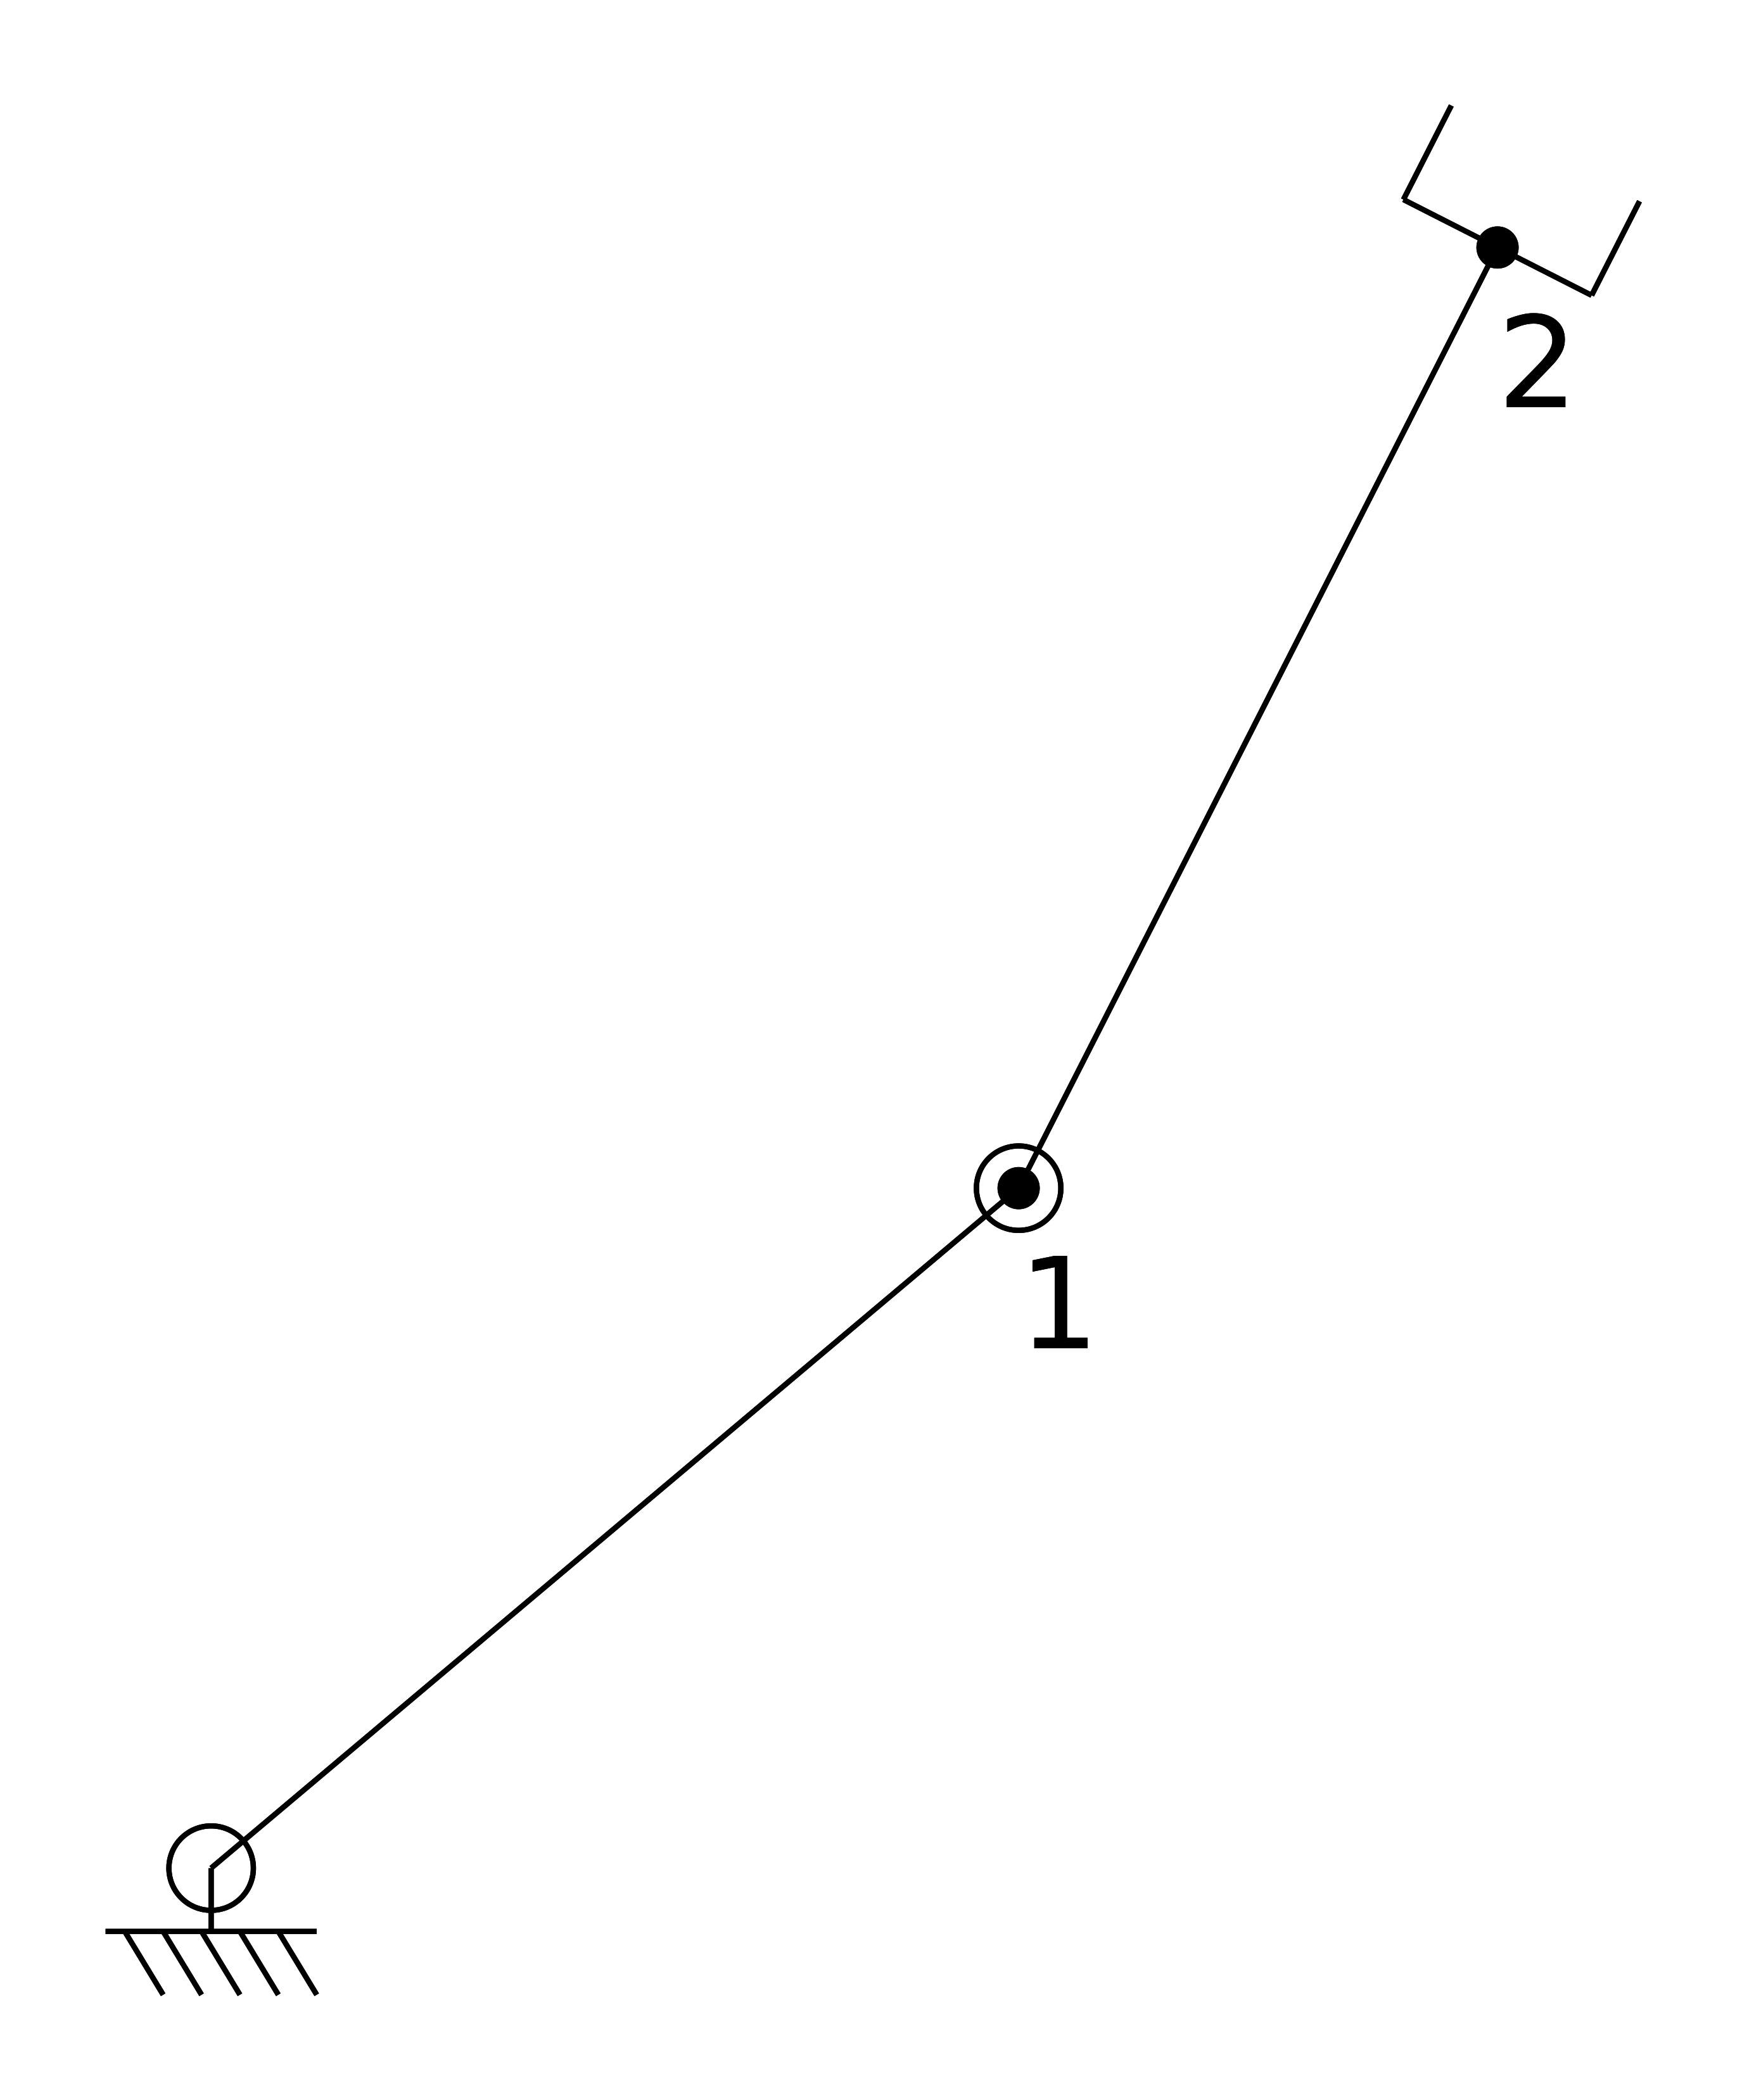
\includegraphics[scale=0.05]{generated_figures/code_1_J_end.png}
        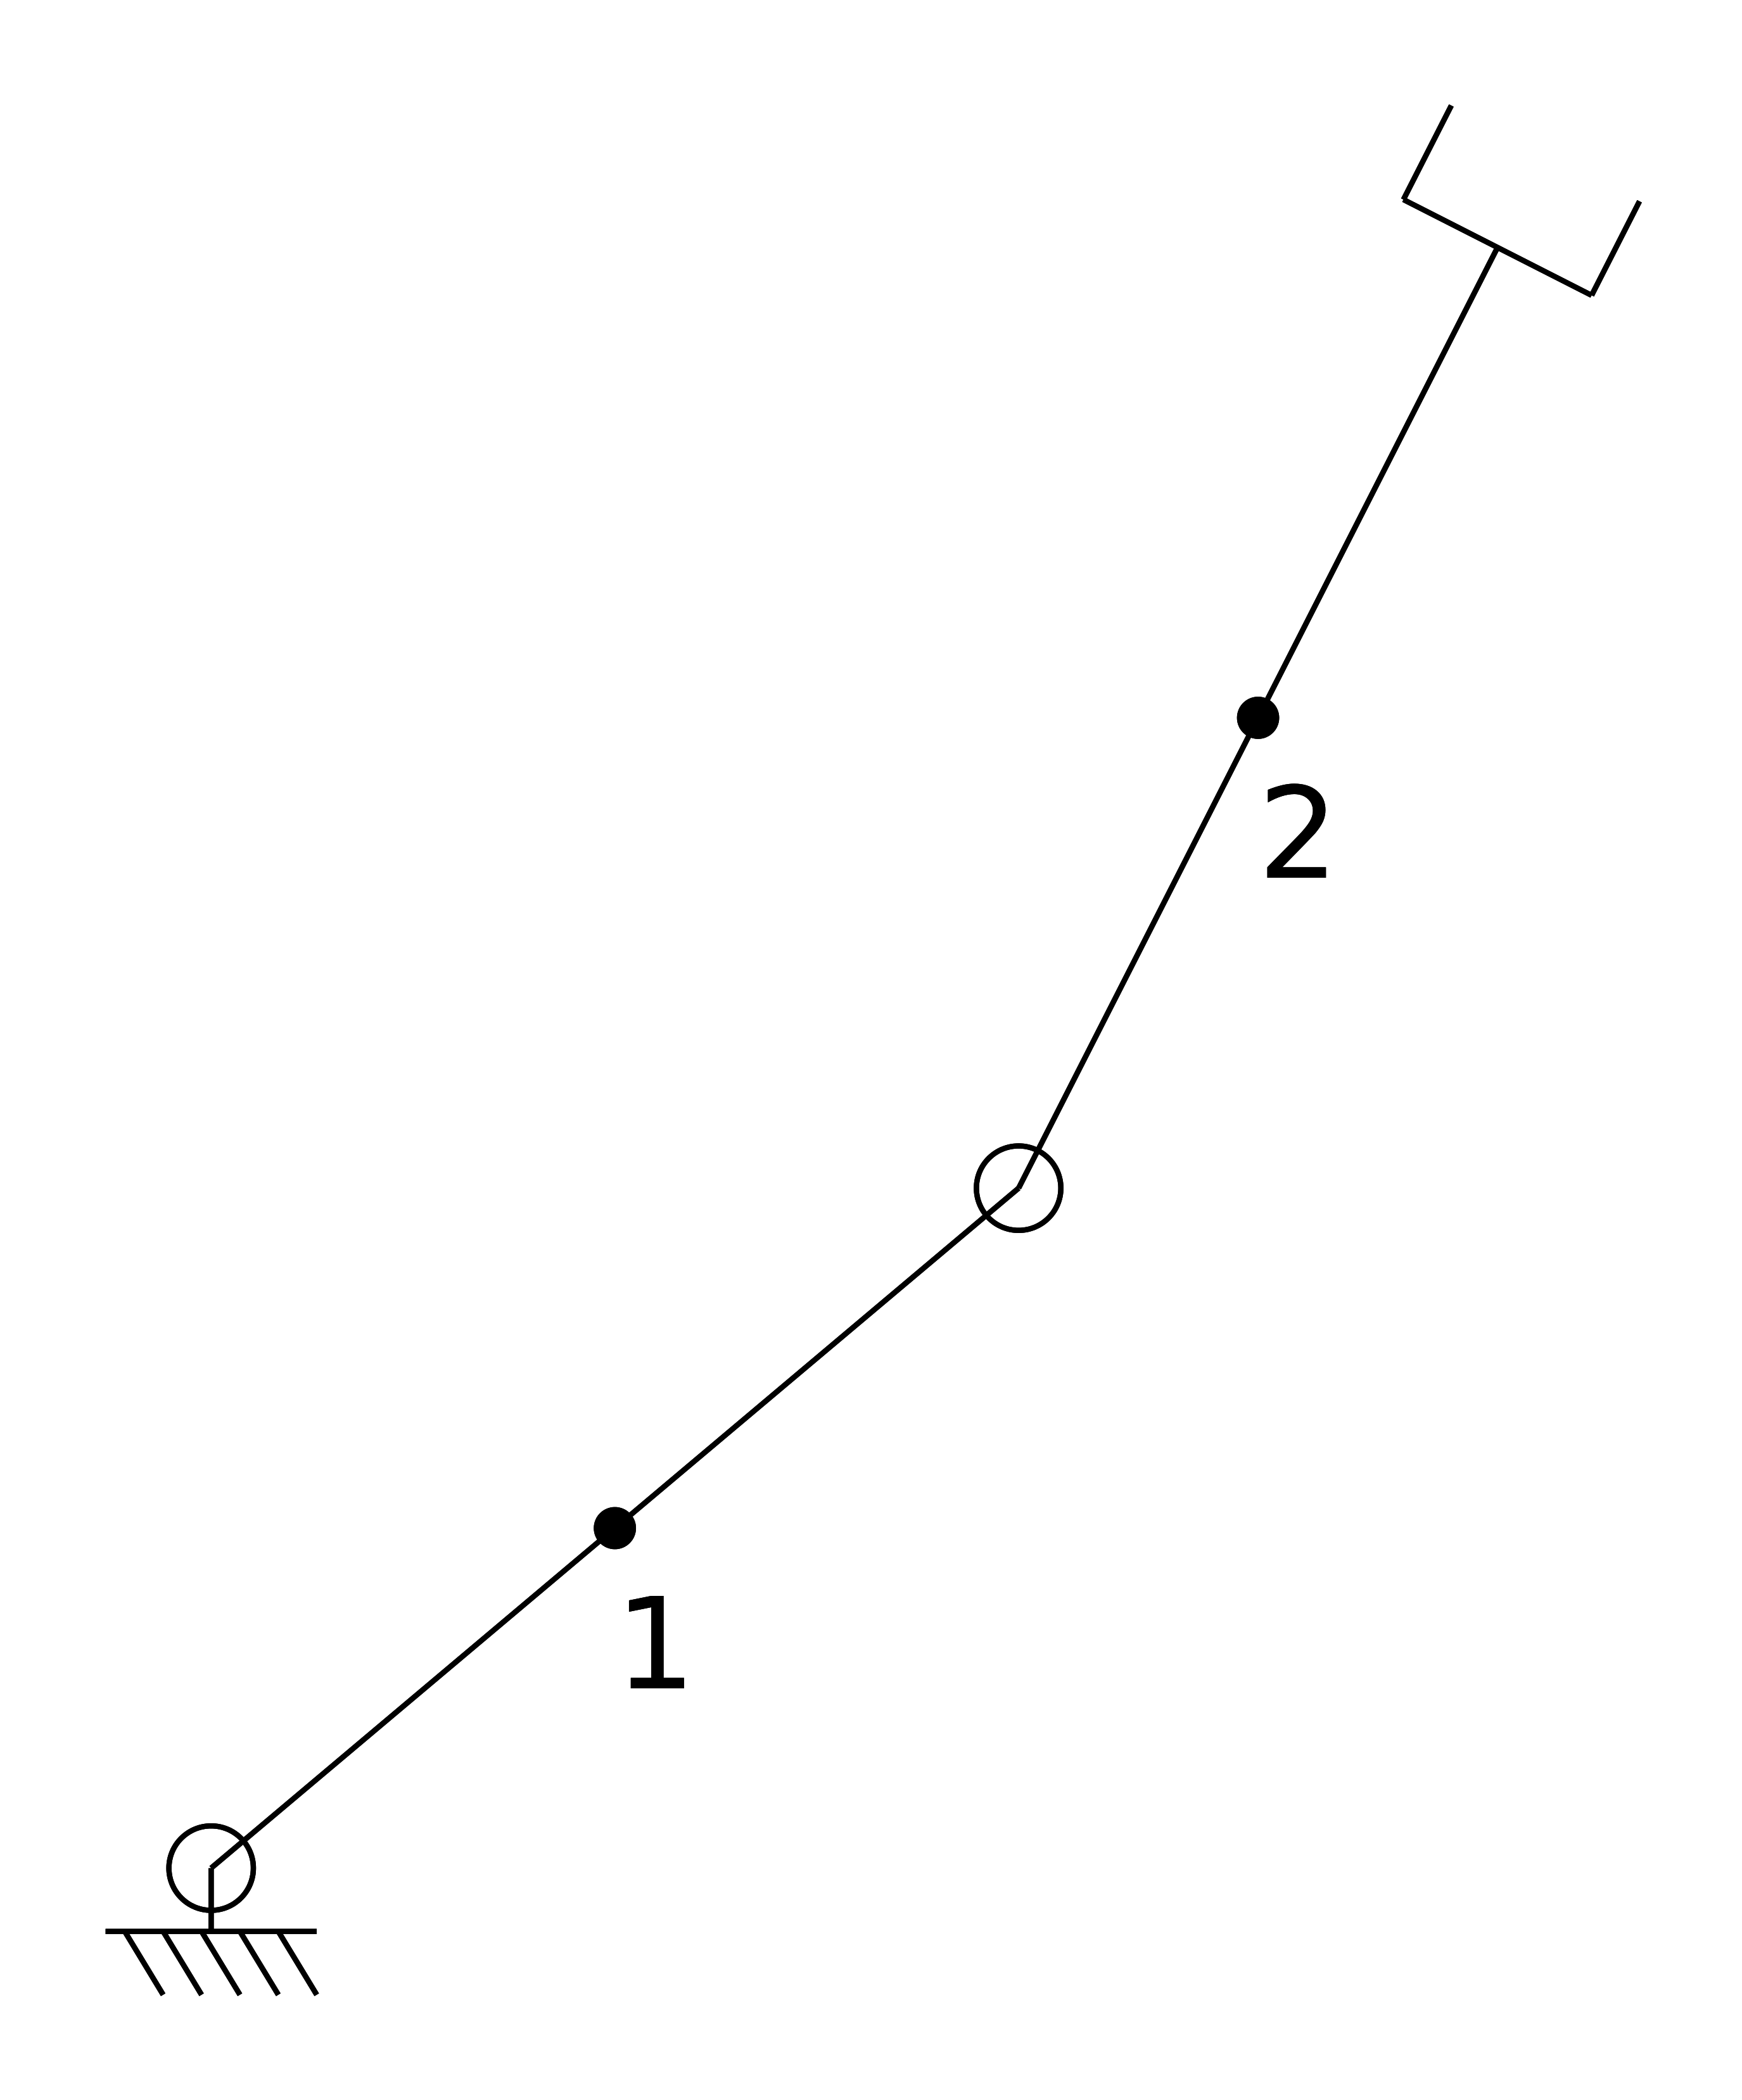
\includegraphics[scale=0.05]{generated_figures/code_1_J_com.png}
        \end{center}
        \begin{itemize}
        \item \verb!forward_kinematics_RR.py!: As in Exercise 1 from Assignment 1, the forward kinematics to several frames should be filled in. Note: the frames for this problem are a subset of those from the previous assignment. In the code, \verb!H_1_0!, \verb|H_2_0|, and \verb|H_3_0| refer to $H_1^0$, $H_2^0$, and $H_3^0$ respectively (where \frame{0}, \frame{1}, and \frame{2} are shown in the above left figure). \frame{3} is at the end-effector.
        \item \verb!jacobian_link_ends_RR.py!: Jacobian matrices to the end of
        the robot links should be filled in in this problem. In the code,
        \verb!J_END_1! and \verb!J_END_2! refer to the Jacobians to the end of link 1 and 2 respectively
        (i.e., points 1 and 2 in the above middle figure).
        \item \verb!jacobian_coms_RR.py!: Jacobian matrices to the centers of
        the robot links should be filled in in this problem. In the code,
        \verb!J_COM_1! and \verb!J_COM_2! refer to the Jacobians to the center of link 1 and 2 respectively
        (i.e., points 1 and 2 in the above right figure).
        \item \verb!sample_path.py!: This function loads data taken from the
        robot, and draws the path taken by the center and end of each link. You
        should use the functions you have written above to fill in the position
        and velocity of these points.
        \end{itemize}
        After completing these tasks, run the \verb!sample_path.py! function. You
        should see four separate lines, representing the path of the center and end
        of each link. These lines should be formed of arrows, which represent the
        velocity of each of these points. \textbf{Important:} if the arrows are not
        tangent to the path, there is an error in your code! Verify your code is
        correct before continuing. As before, when debugging, remember to use
        simple test cases such as $\begin{bmatrix} 0 \\ 0 \end{bmatrix}$ or $\begin{bmatrix} 0 \\ \frac\pi2 \end{bmatrix}$ to check
        your matrices.

    \textbf{The deliverables for this problem} are the four Python files mentioned above, as well as the resulting figure from running \verb!sample_path.py!. This figure should be saved as \verb!path.png!. Additionally, \verb!sample_path.py! will generate a \verb!results.pkl! file containing the calculated data for each part of the robot. This file will be used for grading, so ensure it is generated correctly.


        \titledquestion{Forces and Gravity Compensation}[25]
Begin by opening the \verb!ex2! directory in your Python environment.
In this exercise, you must use the Jacobians found in the first problem
to compute joint torques which result in forces applied by the robot. This
will involve completing two functions:
\begin{itemize}
\item \verb!get_joint_torques.py!: In this function, you must determine
the joint torques necessary for applying a given force with the end
effector (e.g., centered at the end effector origin in a given
direction with a given magnitude).
\item \verb!get_grav_comp_torques.py!: In this function, you will
compute the joint torques which compensate for the force of gravity on
each part of the robot, given the current joint angles.  Note the
direction and magnitude of acceleration due to gravity is passed into
this function (assume units of m/s$^2$).
\end{itemize}
After completing these functions, run the \verb!sample_torques.py! script.
This script will generate plots of your computed torques for a test run of the robot.
Two figures will be produced: one containing torques for applying a
force with the end effector, and the other containing torques for
compensating for gravity.

\textbf{The deliverables for this problem} are the two completed Python files above,
as well as the resulting figures from running \verb!sample_torques.py!. These
figures will be automatically saved as \verb!torques_ee.png! and \verb!torques_grav_comp.png!,
respectively. Please also include copies of these figures in your writeup!

Additionally, the \verb!sample_torques.py! script will save your computed torques
as pickle files (\verb!tau_desired_force.pkl! and \verb!tau_grav_comp.pkl!).
These will be used for grading purposes, so ensure they are generated correctly.

Note: The \verb!sample_torques.py! script uses functions from the \verb!ex1! directory.
Make sure your Python environment is set up correctly to access these functions.

    \titledquestion{Submission}

    To submit, run \verb!create_submission.py!.  It will first run \verb!autograder.py! to confirm your submitted files run without error and then produce a zip file \verb|submission.zip| containing your \verb!ex1! and \verb!ex2! folders. Rename that file to \verb!<andrew_id>.zip! and upload it to Gradescope.

\end{questions}

\begin{submissionChecklist}
        \item Create a PDF of your answers to the written questions with the name \verb!<andrew_id>.pdf! and submit it to Gradescope.
        \item Run \verb!autograder.py! and confirm it reports no failures.
        \item Run \verb!create_submission.py! in the python terminal.
        \item Rename \verb|submission.zip| and upload \verb!<andrew_id>.zip! to Gradescope.
        \item Coding questions are autograded, with no limit on number of submissions within the mandated deadline.
	\end{submissionChecklist}

\end{document}
